\section{Generación y puesta en marcha de la base de datos}

El diagrama final de la base de datos quedaría como puede observarse en la figura \ref{fig:db-design}.
\begin{figure}[ht]
    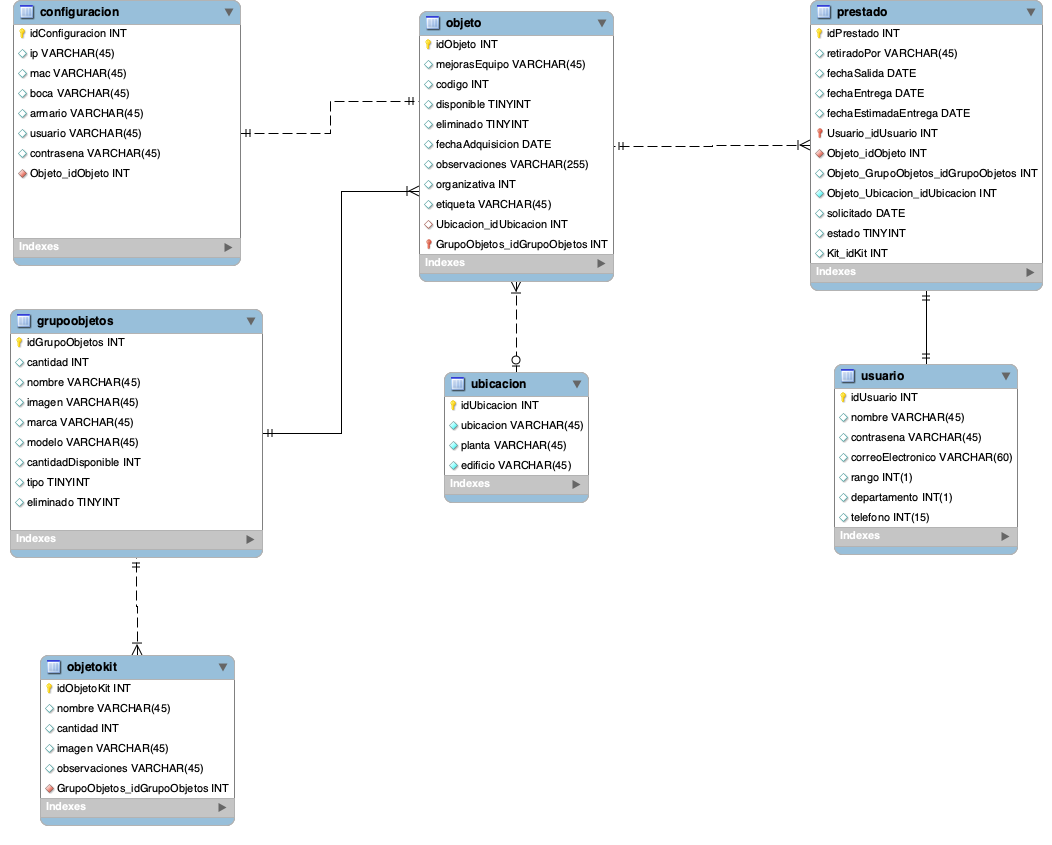
\includegraphics[width=\textwidth,height=\textheight,keepaspectratio]{db_design.png}
    \caption{Diseño final de la base de datos}\label{fig:db-design}
\end{figure}
Se generará el script ``.sql'' para poder crear la base de datos.
\\Esta configuración se basará únicamente en la sección de código que se añadirá dentro del docker-compose.yml.
\\Se añade la versión de docker-compose \cite{docker-compose-create} a utilizar:

\begin{verbatim}
version: "3.9"
\end{verbatim}

Se creará el apartado ``services'':

\begin{verbatim}
    services:
\end{verbatim}

Se añade el primer contenedor, en este caso, el de la base de datos:

\begin{verbatim}
    db:
    container_name: inventarium_sql
    image: mariadb:10.7.1-focal
    ports:
      - "3306:3306"
    volumes:
      - ./dump:/docker-entrypoint-initdb.d
      - persistent:/var/lib/mysql
    networks:
      - default
    environment:
      MYSQL_DATABASE: ualinventarium
      MYSQL_USER: ualinventarium
      MYSQL_PASSWORD: contraseñasecreta
      MYSQL_ROOT_PASSWORD: contraseñasecreta
\end{verbatim}
\begin{itemize}
    \item \textbf{db}: Este es el nombre que se le ha puesto como referencia para docker-compose.
    \item \textbf{container\_name}: Es el nombre que tendrá el contenedor que se vaya a desplegar.
    \item \textbf{image}: La imagen utilizada, es decir, la ``máquina virtual'' que se irá a levantar. En este caso es una máquina virtual de MariaDB.
    \item \textbf{ports}: Los puertos que utilizará la máquina, a la izquierda son los que le llegan a la máquina y a la derecha los que salen.
    \item \textbf{volumes}: Esta sección es muy importante ya que aquí se podrán importar archivos en el momento del despliegue del entorno. En este caso se está importando la carpeta ``dump'' donde está el archivo de generación de la base de datos. También se le enlazará el volumen ``persistent'' que se creará más adelante. Esto es para que no se pierdan datos cuando se detenga contenedor ya que los datos de la base de datos, se almacenarán en un sitio externo.
    \item \textbf{networks}: Aquí pueden añadirse las redes que manejará el contenedor. En este caso es la default.
    \item \textbf{environment}: Dentro de environments se podrán definir variables que se necesiten en el momento del despliegue del contenedor. En este caso se definirá el nombre de la base de datos, el usuario junto a su contraseña y la contraseña del usuario root.
\end{itemize}
\begin{verbatim}
    phpmyadmin:
    container_name: inventarium_php_adm
    image: phpmyadmin:5.1
    links:
      - db:db
    ports:
      - 8000:80
    environment:
      MYSQL_USER: user
      MYSQL_PASSWORD: user
      MYSQL_ROOT_PASSWORD: user
    networks:
      - default
\end{verbatim}
Este despliegue es para phpmyadmin, el gestor de la base de datos. Como añadido al punto anterior está el apartado \textbf{links} que ayuda a crear una vinculación de un contenedor con otro. En este caso se le está pasando la información de la base de datos para que trabaje sobre ella.
\begin{verbatim}
volumes:
    persistent: {}
\end{verbatim}
Dentro de la sección \textbf{volumes} se pueden generar volúmenes que se van a utilizar dentro de los contenedores. En este caso se ha creado el volumen ``persistent'' para poder guardar la información que se almacene dentro de nuestra base de datos.
\vspace{\baselineskip}
\\Para levantar la base de datos se ejecutará dentro del directorio donde se ha creado el docker-compose.yml el siguiente comando:
\begin{verbatim}
    sudo docker compose up
\end{verbatim}
Ya con esto estaría la base de datos en funcionamiento.
\vspace{\baselineskip}
\begin{tcolorbox}
    [colback=green!5!white,colframe=green!75!black,fonttitle=\bfseries,title=¿Cómo comprobamos los resultados?]
    Visual Studio Code realiza una \textbf{tunelización de los puertos} a partir de la conexión SSH. Es decir, habilita redireccionamientos de puertos para poder ir viendo los resultados en la máquina. Esto resulta de gran ayuda ya que no hay que realizar una configuración en la máquina de apertura de puertos para poder ir trabajando sobre cada una de las aplicaciones existentes ya que el funcionamiento del sistema será interno. Con poder disponer de los puertos HTTP Y HTTPS abiertos no se necesitará más.
\end{tcolorbox}

